\section{Problem Formulation}
%----------------------------------------------------------------------------------------%
Outline:
\begin{itemize}
    \item The resulting joint action influences the evolution of the system;
    \item However, we formulate the MMDP into standard MDP framework, with fully-observable information and joint actions;
    \item two phases policy, due to partially observed information; thus we come up with sub-optimal solution to the Bellman equation; (where the lower and upper bound are analytically obtained)
\end{itemize}

\delete{
    [MMDP, POMDP, DEC-POMDP]
    [1] "Sequential Optimality and Coordination in Multi-agent Systems", Craig Boutilie, 1999
    [2] "Taming Decentralized POMDPs: Towards Efficient Policy Computation for Multi-agent Settings", R.Nair, 2003
}

In this section, we formulate the optimization problem which aims at online optimizing job dispatching decisions of all APs.
This kind of optimization problem falls into multi-agent planning problem, which considers a fully cooperative multi-agent system (MAS) and each agent shares the same utility function \needref{Craig Boutilie, 1999}.

\needref{R.Nair, 2003} introduces DEC-POMDP to characterize the decentralized
We formulate the problem under standard Markov Decision Program (MDP) framework, which

\fixit{
    We describe the system state and policy from a global perspective, where each AP adopts the dispatching policy mapping from the collected global state information.
    Due to the different distributions of \brdelay~for each AP, APs use the stale policy in one interval firstly, and then update their policy at different time slots in an unknown order.
    Therefore, we come up with efficient decentralized online algorithm (polling iterative update), which is upper bounded by 
    At the end of this section, we show that the (polling iterative) solution of the problem suffers from curse of dimensionality and a low-complexity solution is needed.
}

\subsection{System State and Dispatching Policy}
We formulate the multi-agent MDP problem where each AP shares same utility function in a fully cooperative setting and individually takes action to perform.
The system state is selected from the global perspective.
We consider all the APs maintain the same global information, which is collected and updated by broadcast at the beginning of each interval.
As each AP would update its dispatching policy based on the latest broadcast information, the \brdelay{s} in each interval is also taken as a part of state information.
The relationship between \brdelay~and the policy update time points for different APs is depicted in Fig. \ref{fig:brd-trans}.
\begin{definition}[System State]
    The system state at $i$-th \brpoint~is denoted as follows.
    \begin{align}
        \Stat(t_i) \define \Paren{
            \Obsv(t_{i-1}), \Obsv({t_{i}}), \mathcal{D}(t_{i})
        },
    \end{align}
    where $\mathcal{D}(t_{i}) \define \set{D_{1}(t_{i}), \dots, D_{K}(t_{i})}$ denotes the \brdelay~for each AP, $\Obsv(t_{i})$ denotes updated information after receiving the whole broadcasting information, and $\Obsv(t_{i-1})$ denotes the stale information.
\end{definition}

\begin{figure}[ht]
    \centering
    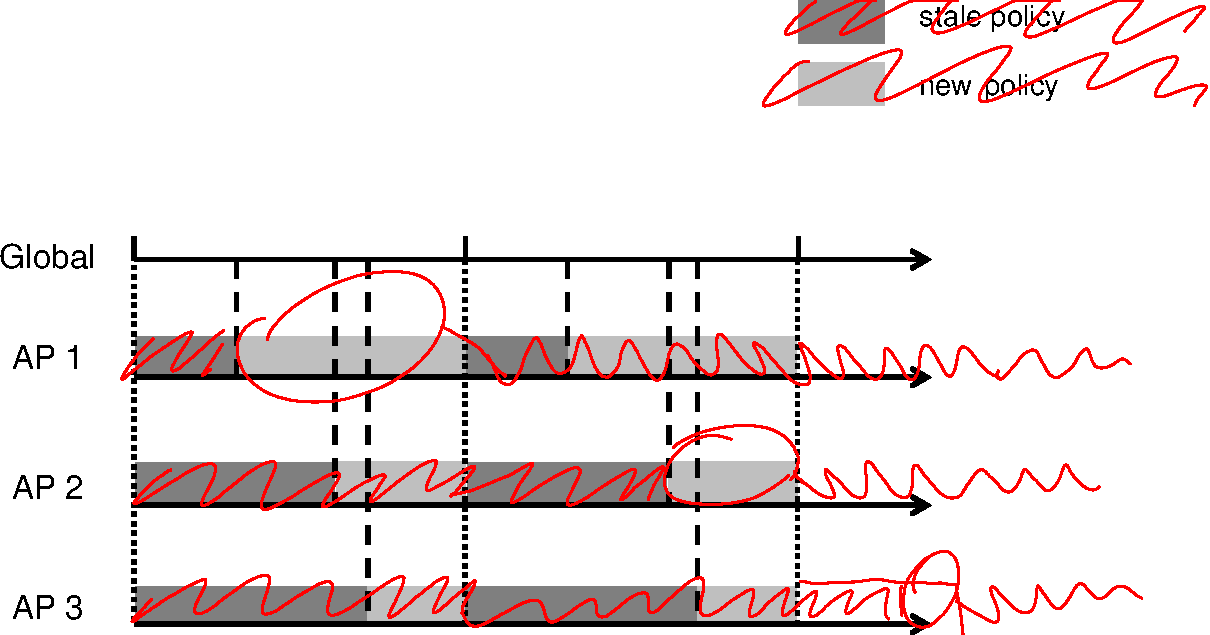
\includegraphics[width=0.80\textwidth]{brd-trans.pdf}
    \caption{Global System Transition with Partial Information-based Dispatching Decision}
    \label{fig:brd-trans}
\end{figure}

Based on the two phases of global broadcast information in the system state, the global joint policy of all APs is defined as follows.
\fixit{Independent Action space by Cartesian product, e.g. $A \times A \times \dots \times A$;}
\begin{definition}[Joint Dispatching Policy]
    The joint dispatching policy $\Policy(\Stat(t_{i}))$ over $\Stat(t_{i})$ which is defined with two phases broadcasting information which is given as follows.
    \begin{align}
        \Policy\Paren{\Stat(t_{i})} \define \Brace{
            \Omega_{1}\Paren{\Stat(t_{i})}, \dots, \Omega_{K}\Paren{\Stat(t_{i})}
        },
    \end{align}
    where
    $\Omega_{k}(\Stat(t_{i}))$ denotes the independent policy for the $k$-th AP ($\forall k\in\apSet$), whose definition is given as follows.
    \begin{align}
        \Omega_{k}\Paren{\Stat(t_{i})} \define
        \begin{cases}
            \tilde{\Omega}_{k}( \Obsv(t_{i-1}) ), &n < D_{k}(t_{i})
            \\
            \tilde{\Omega}_{k}( \Obsv(t_{i}) ), &n \geq D_{k}(t_{i})
        \end{cases},
    \end{align}
    where $n$ denotes the index of time slot in the $i$-th interval.
\end{definition}

We note that with the dispatching policy given, the arrival distribution $A_{k,j}$ of the $j$-th job on the $k$-th AP ($\forall k\in\apSet, j\in\jSpace$) is further split onto different Edge Servers.
The split job arrival distributions are still i.i.d Bernoulli distributions with arrival probability as 
$\tilde{\lambda}^{(k)}_{m,j}(t_{i}) \define \lambda_{k,j} I[\omega_{k,j}(t_i) = m]$ ($\forall m\in\esSet$), where $I[\cdot]$ is the indicator function.
%----------------------------------------------------------------------------------------%

\subsection{The Optimization Problem}
We propose the jobs dispatching optimization problem with the target to minimize \emph{average response time} of all offloaded jobs in MEC system.
The \emph{average response time} is composed of uploading time from APs to edge servers, and queueing-and-service time on corresponding edge server. According to \emph{Little's Law}, the average response time of all jobs is equally as average number of jobs in system.
        
\accept{
    Due to the periodic information broadcasting, we collect the cost for counting numbers at the pace of broadcasting interval which could be seen as a uniform sampling of original process based on timeslot scale.
}
Besides the cost counted for job response time, we further add penalty on jobs rejection on edge servers when the job submission is over the queue capacity limit. The penalty will be counted at the end of each broadcast interval.
The cost function of this problem is given as follows.
\begin{align}
    g\Paren{\Stat(t_{i}), \Policy(\Stat(t_{i}))} \define
        &\sum_{k\in\apSet} \sum_{m\in\esSet} \sum_{j\in\jSpace} \vec{R}^{(k)}_{m,j,\xi}(t_{i})~+
        \nonumber\\
        &\sum_{m\in\esSet} \sum_{j\in\jSpace} \Brace{L_{m,j}(t_{i}) + \beta \cdot \mat{I}[L_{m,j}(t_{i})=L_Q]},
\end{align}
where $\beta$ is the weight factor for job rejection penalty ($\beta \in (0,1)$).
        
The definition for global optimization problem is given as follows.
\begin{problem}[Global Job Dispatching Problem]
    \begin{align}
        \min_{\Policy} \lim_{T \to \infty}
            \mathbb{E}_{\Policy}
                \Bracket{\sum_{i=1}^{T} \gamma^{i-1} g\Paren{\Stat(t_{i}), \Policy(\Stat(t_{i}))}|\Stat(t_1)},
    \end{align}
    where the cost is collected with a discount factor $\gamma$.
\end{problem}
\delete{and $\Policy$ is optimized policy globally always with full-state information available.}
According to \cite{sutton1998introduction}, the above problem could be solved by the following \emph{Bellman's equation}:
\begin{align}
    V\Paren{\Stat(t_{i})} =~&g\Paren{\Stat(t_{i})} + \gamma \min_{\Policy(\Stat(t_{i}))}
        \nonumber\\
        &\sum_{\Stat(t_{i+1})} \Pr\Brace{ \Stat(t_{i+1})|\Stat(t_{i}), \Policy(\Stat(t_{i})) } \cdot V\Paren{\Stat(t_{i+1})}.
    \label{sp_0}
\end{align}

\delete{
    the APs update their own policy independently in a decentralized manner.
    The decentralized manner implies each AP only update the policy of itself, and consider other APs' policy fixed in the environment.
}
\delete{
    The formulation of sub-problem is given as follows.
    \begin{problem}[Decentralized Cooperative Job Dispatching sub-Problem]
        We have total $K$ sub-problems and the definition for the $k$-th sub-problem is given as follows ($\forall k\in\apSet$).
        \begin{align}
            \min_{\tilde{\Omega}_k} \lim_{T \to \infty}
                \mathbb{E}_{\Policy'_{k}}
                    \Bracket{\sum_{i=1}^{T} \gamma^{i-1} g\Paren{\Stat(t_{i}), \Policy'_{k}(\Stat(t_{i}))}|\Stat(t_1)},
        \end{align}
        where $\Policy'_{k}(\Stat(t_{i})) \define \set{\Omega_{1}, \dots, \Omega_{k}(\Stat(t_{i})), \dots, \Omega_{K}}$.
    \end{problem}
    The corresponding Bellman's Equation for the $k$-th sub-problem is given as follows.
    \begin{align}
        &V\Paren{\Stat(t_{i})} = g\Paren{\Stat(t_{i})}
        \nonumber\\
        &~~~~+ \gamma \min_{\tilde{\Omega}_{k}(\Obsv(t_{i}))} \Pr\Brace{ \Stat(t_{i+1})|\Stat(t_{i}), \Policy'_{k}(\Stat(t_{i})) } \cdot V\Paren{\Stat(t_{i+1})}.
        \label{sp_k}
    \end{align}
    % $\tilde{\Omega}_{k}(\Obsv(t_{i}))$ is the component of $\Policy(\Obsv(t_{i}))$.
    \begin{remark}
        Assume that we solve the sub-problems following the order of index of AP set, and then substitute the solution to the $k$-th problem to the $(k+1)$-th problem ($\forall k\in\apSet$).
        Apparently, we could achieve a sub-optimal solution of all APs which is upper bounded by the solution to the original problem.
    \end{remark}
}

To better analyze the optimization structure of the problem, we decouple the transition function. The expression of transition function in Eqn. \ref{sp_0} is given as follows.
\begin{lemma}[Transition Function Decoupling]
    The transition function in Bellman's equation could be decoupled on states of APs and edge servers, which will facilitate the approximated value function expression in the following section.
    The decoupled transition function for Eqn. \ref{sp_0} is given as follows.
    \begin{align}
        & \Pr\Brace{ \Stat(t_{i+1})|\Stat(t_{i}), \Policy'_{k}(\Stat(t_{i})) }
        \nonumber\\
        =& \Pr\Brace{ \Obsv(t_{i+1})|\Obsv(t_{i}), \Policy'_{k}(\Stat(t_{i})), D_{k}(t_{i}) } \times \Pr\{\mathcal{D}(t_{i+1})\}
        \nonumber\\
        =& \prod_{k\in\apSet}\prod_{m\in\esSet}\prod_{j\in\jSpace}
                \Pr\Brace{
                    \vec{R}^{(k)}_{m,j}(t_{i+1}) | \vec{R}^{(k)}_{m,j}(t_{i}),
                    \Policy'_{k}(\Stat(t_{i})), D_{k}(t_{i})
                }
                \times  
            \nonumber\\
            & \prod_{m\in\esSet}\prod_{j\in\jSpace}
                \Pr\Brace{
                    Q_{m,j}(t_{i+1})|Q_{m,j}(t_{i}), \mathcal{R}(t_{i}), \Policy'_{k}(\Stat(t_{i})), D_{k}(t_{i})
                }.
    \end{align}
\end{lemma}
\begin{proof}
    Proof deleted.
\end{proof}

The first part denotes the state transition on AP.
Denote as
\begin{align}
    \Pr\Brace{
        \vec{R}^{(k)}_{m,j}(t_{i+1}) | \vec{R}^{(k)}_{m,j}(t_{i})
    } \sim \vecG{\Theta}^{(k)}_{m,j}(t_{i+1}),
\end{align}
where $\vecG{\Theta}^{(k)}_{m,j}(t_{i+1}) \define [\vecG{\theta}^{(k)}_{m,j,0}(t_{i+1}), \dots, \vecG{\theta}^{(k)}_{m,j,\Xi}(t_{i+1})]$.
Given that the uploading process could be depicted by the series of counters, we further have
$\Pr\Brace{R^{(k)}_{m,j,\xi+1}(t_{i+1})|R^{(k)}_{m,j,\xi}(t_{i})} \sim \vecG{\theta}^{(k)}_{m,j,\xi}(t_{i+1})$ ($\forall \xi=0,\dots,\Xi$).
Then we could express the distribution with a transition matrix as:
\begin{align}
    \vecG{\Theta}^{(k)}_{m,j}(t_{i+1}) \define \hat{\Gamma}^{(k)}_{m,j}\Paren{\Policy(\Stat(t_i)) }\vecG{\Theta}^{(k)}_{m,j}(t_{i}),
\end{align}
where transition matrix $\hat{\Gamma}^{(k)}_{m,j}$ is a \emph{block matrix}, whose element is transition matrix $\Gamma^{(k)}_{m,j,\xi}$ for the distribution on the series of counters. The definition is given as follows.
\begin{align}
    &\vecG{\theta}^{(k)}_{m,j,\xi+1}(t_{i+1}) \define
    \nonumber\\
    &\begin{cases}
        ( \Gamma^{(k)}_{m,j,\xi} \dots \Gamma^{(k)}_{m,j,\xi-N} ) \times \vecG{\theta}^{(k)}_{m,j,\xi-N-1}(t_i), &{\xi \geq N}
        \\
        ( \Gamma^{(k)}_{m,j,\xi} \dots \Gamma^{(k)}_{m,j,1} ) \times \vecG{\theta}^{(k)}_{m,j,0}(t_i), &{\xi < N}
    \end{cases},
\end{align}
where $\vecG{\theta}^{(k)}_{m,j,0}(t_{i}) \sim \text{Bernoulli}(\tilde{\lambda}^{(k)}_{m,j}(t_i))$, and transition matrix $\Gamma^{(k)}_{m,j,\xi}$ is time-invariant and defined as follows.
\begin{align}
    \Gamma^{(k)}_{m,j,\xi} = 
    \begin{bmatrix}
        &0 \\
        &p^{(k)}_{m,j,\xi} &\bar{p}^{(k)}_{m,j,\xi} \\
        &(p^{(k)}_{m,j,\xi})^2 &2(p^{(k)}_{m,j,\xi}\bar{p}^{(k)}_{m,j,\xi}) &(\bar{p}^{(k)}_{m,j,\xi})^2 \\
        % &(p^{(k)}_{m,j,\xi})^3 &3(p^{(k)}_{m,j,\xi})^2(\bar{p}^{(k)}_{m,j,\xi}) &3(p^{(k)}_{m,j,\xi})(\bar{p}^{(k)}_{m,j,\xi})^2 &(p^{(k)}_{m,j,\xi})^3 \\
        &\dots &\dots &\dots &\dots
    \end{bmatrix}^T,
\end{align}
where $p^{(k)}_{m,j,\xi} \define \Pr\{U^{(k)}_{m,j} < (\xi+1) | U^{(k)}_{m,j}>\xi\}$ and $\bar{p}^{(k)}_{m,j,\xi} = 1 - p^{(k)}_{m,j,\xi}$.
And $\hat{\Gamma}^{(k)}_{m,j}$ is an off-diagonal block matrix plus the horizontal part w.r.t $\vecG{\theta}^{(k)}_{m,j,0}$, with other entries as zero.

The second part denotes the state transition on edge servers.
Denote
\begin{align}
    \Pr\Brace{ Q_{m,j}(t_{i+1})|Q_{m,j}(t_{i}), \mathcal{R}(t_{i}) } \sim \vecG{\nu}_{m,j}(t_{i}).
\end{align}
We notice that the job arrival distribution $\vecG{\beta}_{m,j}(t_{i})$ is given by $\mathcal{R}(t_{i})$, and the departure rate in one slot is deterministic as $1/N$.
Thus the expectation of $\vecG{\beta}$ would be always far more smaller than $1$ as composed of all $K$ AP nodes.
We take approximation on $\vec{\beta}$ as Bernoulli distribution in each time slot that $\vecG{\beta}(t_{i,n}) \triangleq [\beta^{(0)}_{m,j}(t_{i,n}), \beta^{(1)}_{m,j}(t_{i,n})]$, where
\begin{align}
    \beta^{(1)}_{m,j}(t_{i,n}) &\define \sum_{k\in\mathcal{K}} \sum_{\xi=0,\dots,\Xi-1} \mathbb{E}[\vecG{\rho}^{(k,+)}_{m,j,\xi}(t_{i,n})]
    \label{eqn_0}
    \\
    \vecG{\rho}^{(k,+)}_{m,j,\xi}(t_{i,n}) &\define \tilde{\Gamma}^{(k)}_{m,j,\xi} \times \vecG{\theta}^{(k)}_{m,j,\xi}(t_{i,n})
    % \label{eqn_1}
    \\
    \beta^{(0)}_{m,j}(t_{i,n}) &= 1-\beta^{(1)}_{m,j}(t_{i,n})
    % \label{eqn_2}
\end{align}
And we could obtain the time-variant transition matrix composed of multiple transition matrix $P_{m,j}(\vecG{\beta}(t_{i,n}))$ in all the time slots in $i$-th interval as follows.
\begin{align}
    \vecG{\nu}(t_{i,n+1}) &= P_{m,j}\Paren{\vecG{\beta}(t_{i,n})} \vecG{\nu}(t_{i,n})
    % \label{eqn_3}
    \\
    \vecG{\nu}(t_{i+1}) &= \prod_{n=0,\dots,N-1} P_{m,j}\Paren{\vecG{\beta}(t_{i,n})} \vecG{\nu}(t_{i}),
    \label{eqn_4}
\end{align}
%FIXME: could/should we give explicit definition for $P_{m,j}$ ?
% where
% \begin{align}
%     \Paren{ P_{m,j}(\vecG{\beta}(t_{i,n})) }_{} \define 
%     \begin{cases}
%         , &\eta_{m,j} = 1
%         \\
%         , &\eta_{m,j} > 1
%     \end{cases}
% \end{align}

However, after the state decomposition, the action space would still be exponentially expanded with respect to the number of APs and edge servers.
We could not use traditional \emph{policy iteration} or \emph{value iteration} algorithm \cite{sutton1998introduction} for unacceptable computational complexity.
\st{And we come up with an algorithm which could solve all $K$ sub-problems to achieve a global solution.}
So in next section, to alleviate curse of dimensionality, we introduce baseline dispatching policy to approximate the value function, and then carry out one-step iteration \st{in a polling manner} to obtain a better value function approximation.
%----------------------------------------------------------------------------------------%